% Source: Code/RADAR_web/docs/figures/fig_topology.tex
\documentclass[border=5pt]{standalone}
\usepackage{tikz}
\usetikzlibrary{arrows.meta,positioning}
\usepackage{xcolor}

\definecolor{garnet}{HTML}{73000A}
\definecolor{black90}{HTML}{363636}
\definecolor{atlantic}{HTML}{466A9F}
\definecolor{horseshoe}{HTML}{65780B}

\begin{document}
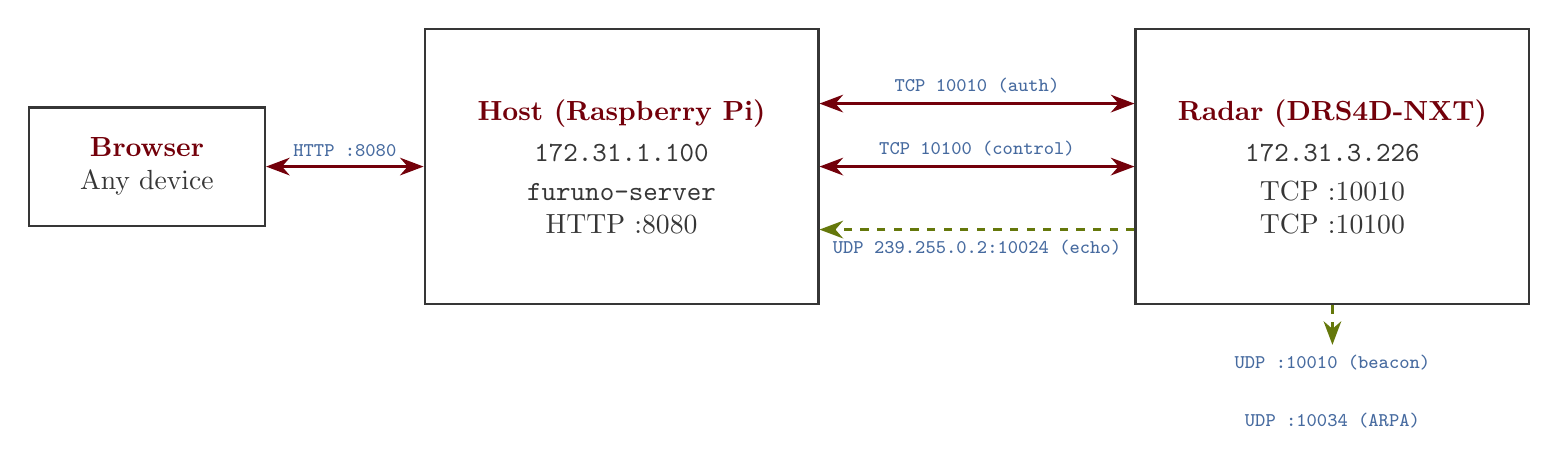
\begin{tikzpicture}[
    node distance=4cm,
    box/.style={draw, thick, minimum width=5cm, minimum height=3.5cm, align=center, color=black90},
    port/.style={font=\ttfamily\scriptsize, color=atlantic},
    arrow/.style={-{Stealth[length=3mm]}, thick, color=garnet},
    biarrow/.style={{Stealth[length=3mm]}-{Stealth[length=3mm]}, thick, color=garnet},
    mcast/.style={-{Stealth[length=3mm]}, thick, dashed, color=horseshoe},
]

% Host box
\node[box] (host) {
    \textbf{\color{garnet}Host (Raspberry Pi)}\\[0.3em]
    \texttt{172.31.1.100}\\[0.2em]
    \texttt{furuno-server}\\
    HTTP :8080
};

% Radar box
\node[box, right=4cm of host] (radar) {
    \textbf{\color{garnet}Radar (DRS4D-NXT)}\\[0.3em]
    \texttt{172.31.3.226}\\[0.2em]
    TCP :10010\\
    TCP :10100
};

% Connection arrows
\draw[biarrow] ([yshift=0.8cm]host.east) -- ([yshift=0.8cm]radar.west)
    node[midway, above, port] {TCP 10010 (auth)};

\draw[biarrow] ([yshift=0cm]host.east) -- ([yshift=0cm]radar.west)
    node[midway, above, port] {TCP 10100 (control)};

\draw[mcast] ([yshift=-0.8cm]radar.west) -- ([yshift=-0.8cm]host.east)
    node[midway, below, port] {UDP 239.255.0.2:10024 (echo)};

% Broadcast below
\node[port, below=0.5cm of radar] (bcast) {UDP :10010 (beacon)};
\draw[mcast] (radar.south) -- (bcast);

\node[port, below=0.3cm of bcast] (arpa) {UDP :10034 (ARPA)};

% Browser
\node[box, minimum height=1.5cm, minimum width=3cm, left=2cm of host] (browser) {
    \textbf{\color{garnet}Browser}\\
    Any device
};
\draw[biarrow] (browser.east) -- (host.west)
    node[midway, above, port] {HTTP :8080};

\end{tikzpicture}
\end{document}
